\PassOptionsToPackage{unicode=true}{hyperref} % options for packages loaded elsewhere
\PassOptionsToPackage{hyphens}{url}
%
\documentclass[]{article}
\usepackage{lmodern}
\usepackage{amssymb,amsmath}
\usepackage{ifxetex,ifluatex}
\usepackage{fixltx2e} % provides \textsubscript
\ifnum 0\ifxetex 1\fi\ifluatex 1\fi=0 % if pdftex
  \usepackage[T1]{fontenc}
  \usepackage[utf8]{inputenc}
  \usepackage{textcomp} % provides euro and other symbols
\else % if luatex or xelatex
  \usepackage{unicode-math}
  \defaultfontfeatures{Ligatures=TeX,Scale=MatchLowercase}
\fi
% use upquote if available, for straight quotes in verbatim environments
\IfFileExists{upquote.sty}{\usepackage{upquote}}{}
% use microtype if available
\IfFileExists{microtype.sty}{%
\usepackage[]{microtype}
\UseMicrotypeSet[protrusion]{basicmath} % disable protrusion for tt fonts
}{}
\IfFileExists{parskip.sty}{%
\usepackage{parskip}
}{% else
\setlength{\parindent}{0pt}
\setlength{\parskip}{6pt plus 2pt minus 1pt}
}
\usepackage{hyperref}
\hypersetup{
            pdfborder={0 0 0},
            breaklinks=true}
\urlstyle{same}  % don't use monospace font for urls
\usepackage{graphicx,grffile}
\makeatletter
\def\maxwidth{\ifdim\Gin@nat@width>\linewidth\linewidth\else\Gin@nat@width\fi}
\def\maxheight{\ifdim\Gin@nat@height>\textheight\textheight\else\Gin@nat@height\fi}
\makeatother
% Scale images if necessary, so that they will not overflow the page
% margins by default, and it is still possible to overwrite the defaults
% using explicit options in \includegraphics[width, height, ...]{}
\setkeys{Gin}{width=\maxwidth,height=\maxheight,keepaspectratio}
\setlength{\emergencystretch}{3em}  % prevent overfull lines
\providecommand{\tightlist}{%
  \setlength{\itemsep}{0pt}\setlength{\parskip}{0pt}}
\setcounter{secnumdepth}{0}
% Redefines (sub)paragraphs to behave more like sections
\ifx\paragraph\undefined\else
\let\oldparagraph\paragraph
\renewcommand{\paragraph}[1]{\oldparagraph{#1}\mbox{}}
\fi
\ifx\subparagraph\undefined\else
\let\oldsubparagraph\subparagraph
\renewcommand{\subparagraph}[1]{\oldsubparagraph{#1}\mbox{}}
\fi

% set default figure placement to htbp
\makeatletter
\def\fps@figure{htbp}
\makeatother


\date{}

\begin{document}

Antoine PLANTIER LP SIGD IOTIA Module Objets Conectés ---

\hypertarget{projet-dobjets-conectuxe9s-ruxe9seau-de-capteurs-communication-lora}{%
\section{Projet d'Objets Conectés : Réseau de capteurs Communication
LoRa}\label{projet-dobjets-conectuxe9s-ruxe9seau-de-capteurs-communication-lora}}

\hypertarget{introduction}{%
\subsection{Introduction}\label{introduction}}

Dans le cadre du Module d'objets conectés, nous avions a faire un projet
metant en oeuvre le protocole de communication \textbf{LoRa}. J'ai
choisis de mettre en place un réseau de communication assurant un relevé
de mesures et leurs utilisations dans un programe python.

Le projet consiste en un noeud collecteur \emph{(Rx/receviver)} qui
receptionne les données envoyées par différents noeuds emeteurs
\emph{(Tx/sender)}. Ces données sont traitées et stoquées par un
programme en python. Celui ci offre différentes actions de traitement et
d'interactions.

\hypertarget{fonctionnement-guxe9nuxe9ral}{%
\subsection{Fonctionnement général}\label{fonctionnement-guxe9nuxe9ral}}

Voici le schéma général du projet.

\begin{figure}
\centering
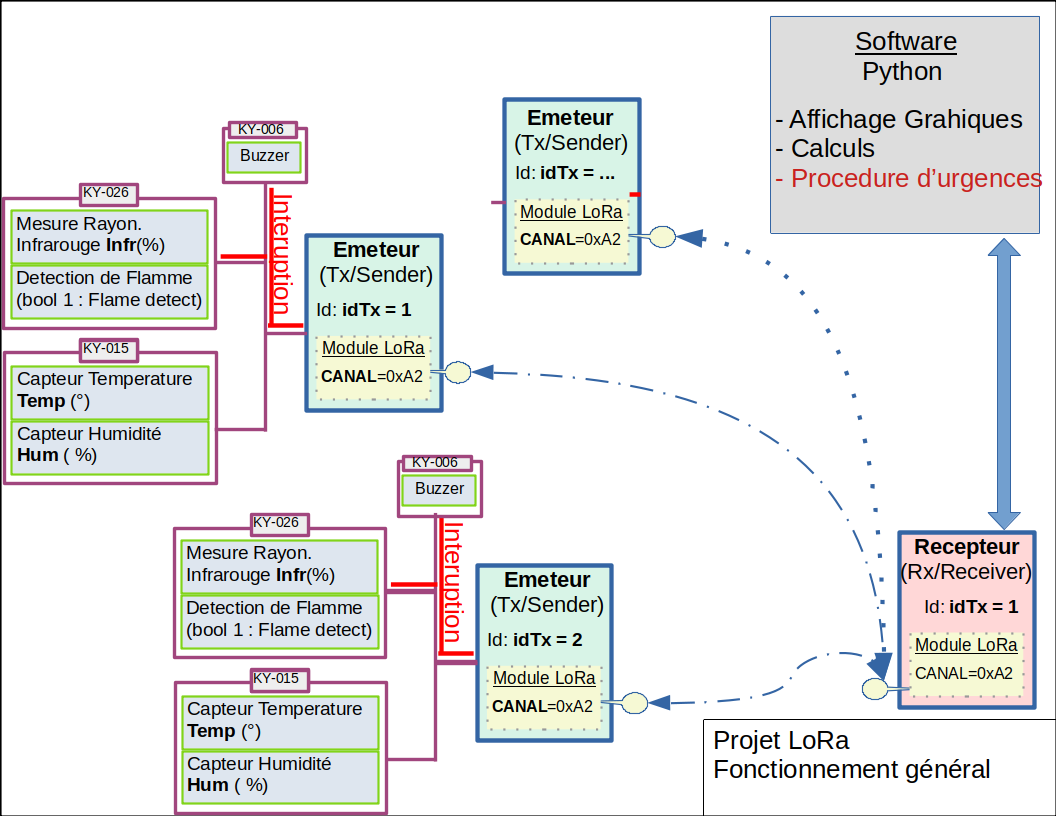
\includegraphics{/home/ourson/cours/ObjCo/Projet/LoRa/src/schem_General.png}
\caption{Projet Général}
\end{figure}

\hypertarget{les-modules-emeteurs-sender-tx}{%
\subsubsection{Les modules Emeteurs : Sender/
TX}\label{les-modules-emeteurs-sender-tx}}

\hypertarget{le-module-recepteur-receiver-rx}{%
\subsubsection{Le module recepteur : Receiver/
Rx}\label{le-module-recepteur-receiver-rx}}

\hypertarget{le-software-en-python}{%
\subsubsection{Le Software en python}\label{le-software-en-python}}

\texttt{\{r,\ attr.source=\textquotesingle{}.numberLines\textquotesingle{}\}\ if\ (TRUE)\ \{\ \ \ x\ \textless{}-\ 1:10\ \ \ x\ +\ 1\ \}}

\end{document}
